\documentclass{article}
% Damit die Verwendung der deutschen Sprache nicht ganz so umst\"andlich wird,
% sollte man die folgenden Pakete einbinden: 
\usepackage[utf8]{inputenc}% erm\"oglich die direkte Eingabe der Umlaute 


\usepackage{amsmath}
\usepackage[T1]{fontenc} % das Trennen der Umlaute
\usepackage{ngerman} % hiermit werden deutsche Bezeichnungen genutzt und 
                     % die W\"orter werden anhand der neue Rechtschreibung 
		     % automatisch getrennt.  
\usepackage{graphicx}

\usepackage{titlesec}
\titleformat{\subsection}{\large\bfseries\sffamily}{}{0pt}{Aufgabe \thesubsection:\quad}

\newcommand{\exercise}[1]{\subsection{#1}}

\begin{document}
\setcounter{section}{1}\setcounter{subsection}{0}

\textbf{Bedingte Wahrscheinlichkeit}

Wir bezeichnen die Wahrscheinlichkeit, dass ein Fußballer F mit links bzw. mit rechts schießt, mit $P\left(L\right)$ bzw. mit $P\left(R\right)$. Ein Schuss von F geht dann mit der Wahrscheinlichkeit $P\left(T\right)$ in's Tor bzw. mit der Wahrscheinlichkeit $P\left(\overline{T}\right)$ nicht in's Tor.

Die \textit{bedingte Wahrscheinlichkeit}, dass der Ball in's Tor geht, unter der Bedingung, dass F mit links geschossen hat, bezeichnen wir mit $P_L\left(T\right)$. Mit diesen Definitionen erhalten wir das folgende Baumdiagramm:

\begin{center}
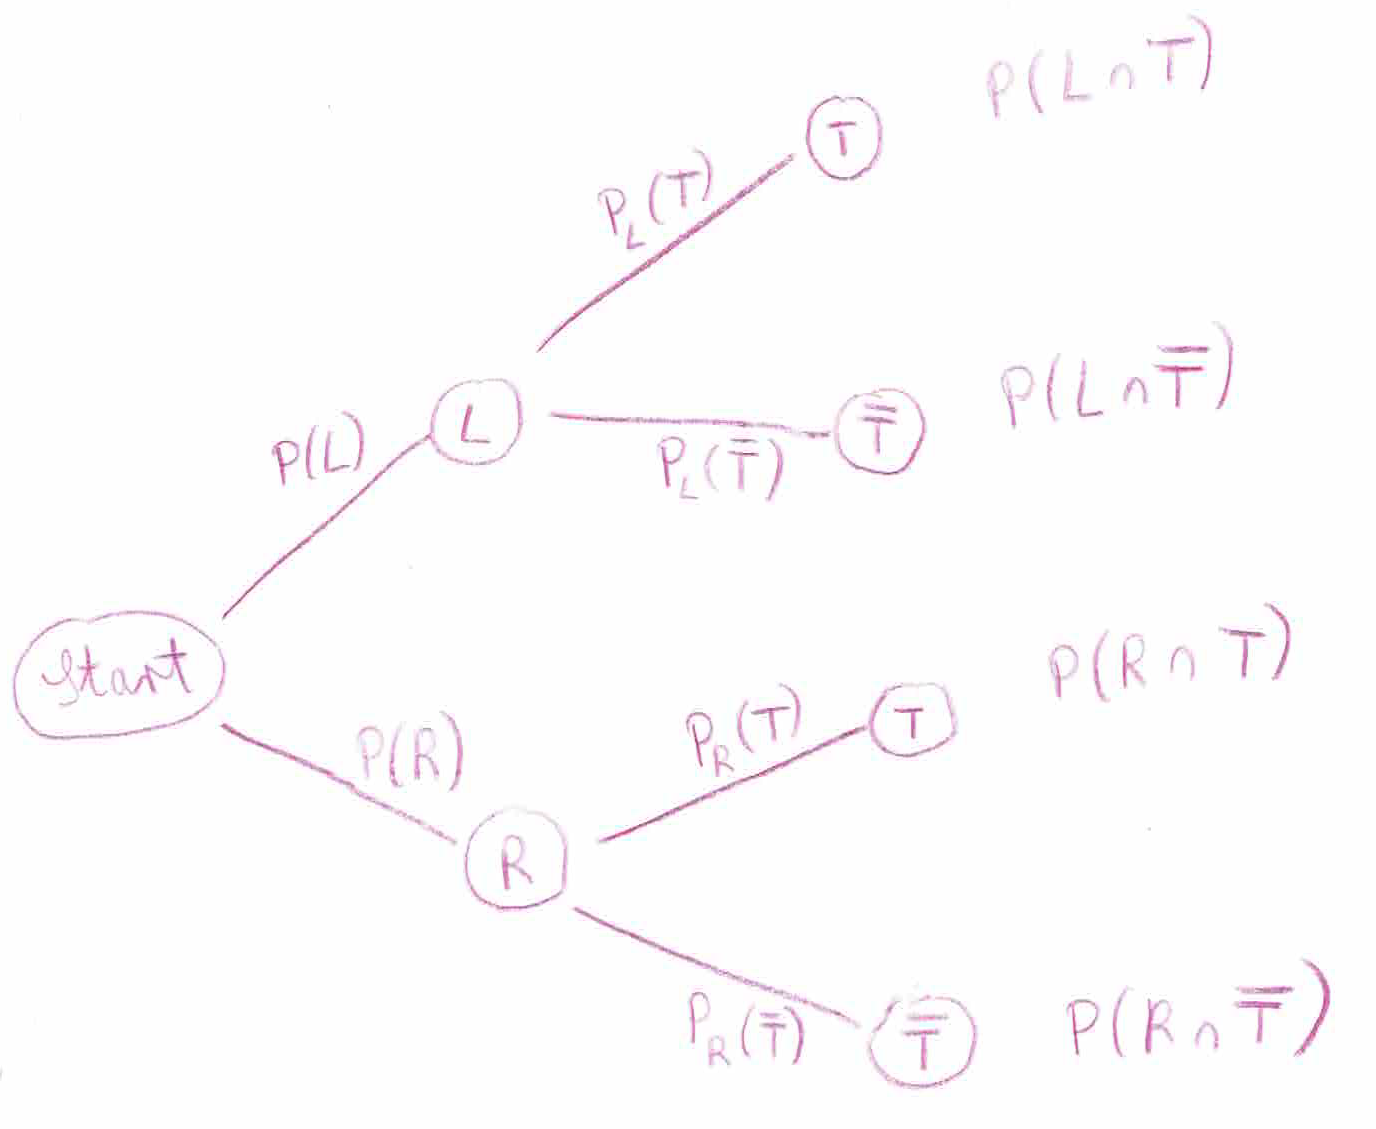
\includegraphics[width=0.7\textwidth]{Baumdiagramm.png}
\end{center}

Nach der 1.Pfadregel ist

\begin{align}
\label{formelone} P\left(L\cap T\right) = P\left(L\right) \cdot P_L\left(T\right) 
\end{align}

\textbf{Aufgabe 1:} Was ergibt sich mit der 1.Pfadregel f\"ur $P\left(L\cap \overline{T}\right)$, $P\left(R\cap T\right)$ und $P\left(R\cap \overline{T}\right)$ ?

L\"osung:
\begin{align}
P\left(L\cap \overline{T}\right) &= P\left(L\right) \cdot P_L\left(\overline{T}\right) \notag \\ 
P\left(R\cap T\right) &= P\left(R\right) \cdot P_R\left(T\right) \notag \\
P\left(R\cap \overline{T}\right) &= P\left(R\right) \cdot P_R\left(\overline{T}\right) \notag   
\end{align}

\vspace{1cm}
Gleichung \eqref{formelone} nach $P_L\left(T\right)$ aufgel\"ost, ergibt:

$$ P_L\left(T\right) = \frac{P\left(L\cap T\right)}{P\left(L\right)}$$

\textbf{Aufgabe 2:} Was ergibt sich f\"ur $P_L\left(\overline{T}\right)$, $P_R\left(T\right)$ und $P_R\left(\overline{T}\right)$ ?

L\"osung:
\begin{align}
P_L\left(\overline{T}\right) &= \frac{P\left(L\cap \overline{T}\right)}{P\left(L\right)} \notag \\
P_R\left(T\right) &= \frac{P\left(R\cap T\right)}{P\left(R\right)} \notag \\
P_R\left(\overline{T}\right) &= \frac{P\left(R\cap \overline{T}\right)}{P\left(R\right)} \notag 
\end{align}

\vspace{1cm}
Mit der 2.Pfadregel ergibt sich:

$$P\left(T\right)\overset{\text{2.Pfadregel}}{=} P\left(L\cap T\right) + P\left(R\cap T\right) \overset{\text{1.Pfadregel}}{=} P\left(L\right) \cdot P_L\left(T\right) + P\left(R\right) \cdot P_R\left(T\right)$$

\textbf{Aufgabe 3:} Was ergibt sich mit der 2.Pfadregel f\"ur $P\left(\overline{T}\right)$?

L\"osung:
$$P\left(\overline{T}\right)\overset{\text{2.Pfadregel}}{=} P\left(L\cap \overline{T}\right) + P\left(R\cap \overline{T}\right) \overset{\text{1.Pfadregel}}{=} P\left(L\right) \cdot P_L\left(\overline{T}\right) + P\left(R\right) \cdot P_R\left(\overline{T}\right)$$

\vspace{1cm}

\textbf{Aufgabe 4:} Sei nun $P\left(L\right) = 0,8$, $P_L\left(T\right) = 0,7$ und $P_R\left(T\right) = 0,4$ gegeben.
Berechnen Sie $P\left(T\right)$ und $P_T\left(L\right)$ !

L\"osung:
\begin{align}
P\left(T\right) &= P\left(L\cap T\right) + P\left(R\cap T\right) \notag \\ &= P\left(L\right) \cdot P_L\left(T\right) + P\left(R\right) \cdot P_R\left(T\right) \notag \\ &= 0,8 \cdot 0,7 + 0,2 \cdot 0,4 \notag \\
&= 0,42 + 0,08 \notag \\
&= 0,5 \notag
\end{align}

\begin{align}
P_T\left(L\right) &= \frac{P\left(L \cap T\right)}{P\left(T\right)} \notag \\
&= \frac{P\left(L\right) \cdot P_L\left(T\right)}{P\left(T\right)} \notag \\
&= \frac{0,8 \cdot 0,7}{ 0,5 } = \frac{0,42}{0,5} = \frac{42}{50} = \frac{84}{100} = 84\% \notag
\end{align}


\end{document}
